\appendix

% ------------------------------------------ CRM Data Facts
\chapter{Appendix: CRM data facts}
\begin{figure}[h]
    \centering
    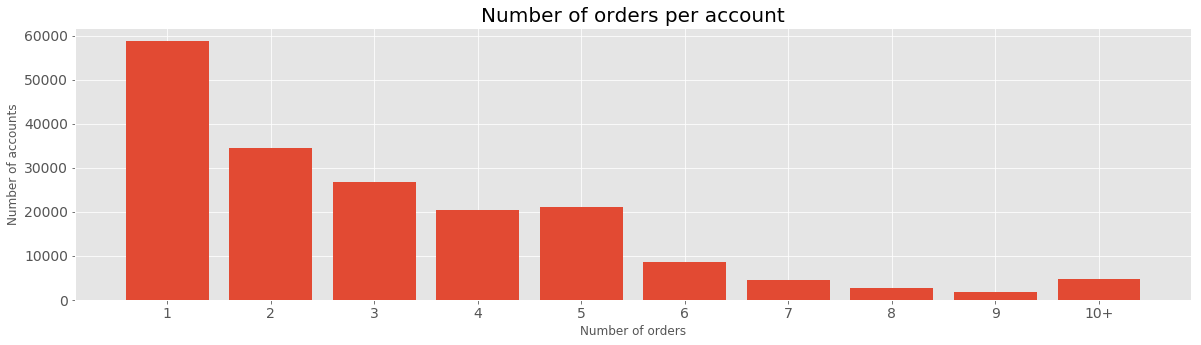
\includegraphics[width=15cm]{images/number_of_orders_per_account.png}
    \caption{Number of orders per accounts}
    \label{fig-annex:orders_per_accounts}
\end{figure}


% ------------------------------------------ Features
\chapter{Features for machine learning}
\label{annex:features-for-ml}

    \begin{tabularx}{1\textwidth}{>{\bfseries}lL} 
        \\\toprule\endfirsthead
        \endhead
        \\ \multicolumn{2}{r}{\itshape continues on next page..}\\\midrule\endfoot
        \bottomrule\endlastfoot
         & \textbf{Account-related features} \\ \midrule
        1.  &   \textbf{account\_order\_id}        \tab   INTEGER     \tab   Number of orders made by the account before \\
        2.  &   \textbf{birth\_year}              \tab   INTEGER     \tab   Year of birth of the account. 0 if year not known \\
        3.  &   \textbf{cumulus}                 \tab   BOOLEAN     \tab   Knowledge of cumulus number for that account \\
        4.  &   \textbf{email}                   \tab   BOOLEAN     \tab   Knowledge of the email for that account \\
        5.  &   \textbf{kunder\_art\_0..6}         \tab   ONE-HOT     \tab   Type of account \\
        6.  &   \textbf{name\_account}            \tab   BOOLEAN     \tab   Is account name null or not \\
        7.  &   \textbf{name\_account\_contact}    \tab   BOOLEAN     \tab   Are account and contact name the same \\
        8.  &   \textbf{name\_contact}            \tab   BOOLEAN     \tab   Is primary contact name null or not \\
        9.  &   \textbf{parent\_account}          \tab   BOOLEAN     \tab   Is an account with childs \\
        10.  &   \textbf{phone}                   \tab   BOOLEAN     \tab   Knowledge of account phone number \\
        11.  &   \textbf{sprache\_0..3}            \tab   ONE-HOT     \tab   Language of account \\
        12.  &   \textbf{tank\_lagergut\_0..9}      \tab   ONE-HOT     \tab   Tank characteristic \\
        13.  &   \textbf{tank\_volumn}             \tab   FLOAT       \tab   Volumn capacity of customer tank \\
    \end{tabularx}
    
    %\pagebreak
    
    \begin{tabularx}{1\textwidth}{>{\bfseries}lL} 
        \\\toprule\endfirsthead
        \endhead
        \\ \multicolumn{2}{r}{\itshape continues on next page..}\\\midrule\endfoot
        \bottomrule\endlastfoot
         & \textbf{Current month features, with \textit{Weather} and \textit{Price}} \\ \midrule
        1.  &   \textbf{menge\_coldays\_0}                           \tab   INTEGER \tab   Last order amount delivered divided by 'nbr\_coldays\_below\_0' \\
        2.  &   \textbf{menge\_coldays\_5}                         \tab   INTEGER \tab   Last order amount delivered divided by 'nbr\_coldays\_below\_5' \\
        3.  &   \textbf{nbr\_coldays\_below\_0}*                     \tab   INTEGER \tab   Number of days with weather below 0 from last order until "today"   \\
        4.  &   \textbf{nbr\_coldays\_below\_5}*                     \tab   INTEGER \tab   Number of days with weather below 5 from last order until "today"   \\
        5.  &   \textbf{nbr\_months\_since\_last\_order}             \tab   FLOAT   \tab   Number of months (float) since previous account order   \\
        6.  &   \textbf{nbr\_weeks\_since\_last\_order}*              \tab   FLOAT   \tab   Number of weeks (float) since previous account order    \\
        7.  &   \textbf{nbr\_weeks\_left\_basedon\_prev}*             \tab   FLOAT   \tab   Number of weeks since last order    \\
        8.  &   \textbf{nbr\_months\_left\_basedon\_prev}*         \tab   FLOAT   \tab   Number of month since last order    \\
        9.  &   \textbf{nbr\_coldays0\_left\_basedon\_prev}*          \tab   INTEGER \tab   Number of days below 0 °C since last order minus number of days below 0 °C between last order and last last order   \\
        10.  &   \textbf{nbr\_coldays5\_left\_basedon\_prev}*         \tab   INTEGER \tab   Number of days below 5 °C since last order minus number of days below 5 °C between last order and last last order   \\
        11.  &   \textbf{nbr\_mengecoldays0\_left\_basedon\_prev}        \tab   FLOAT   \tab   Equation: df['prevmenge\_coldays0']   -  df['menge\_coldays\_0']   \\
        12.  &   \textbf{nbr\_mengecoldays5\_left\_basedon\_prev}        \tab   FLOAT   \tab   Equation: df['prevmenge\_coldays5']   -  df['menge\_coldays\_5']   \\
        13.  &   \textbf{price}                                          \tab   FLOAT   \tab   Current oil price   \\
        14.  &   \textbf{price\_past\_month\_0..9}                   \tab   FLOAT   \tab   Mean of the oil prices for XXX month ago    \\
        15.  &   \textbf{price\_past\_week\_0..3}                \tab   FLOAT   \tab   Mean of the oil prices for XXX week ago \\
        16.  &   \textbf{price\_prev\_diff\_01\_p}                \tab   FLOAT   \tab   Difference in percentage between current price and mean price of one month ago  \\
        17.  &   \textbf{price\_prev\_diff\_12\_p}                \tab   FLOAT   \tab   Difference in percentage between mean price of one month ago and mean price of 2 months ago \\
        18.  &   \textbf{price\_prev\_diff\_23\_p}                \tab   FLOAT   \tab   Difference in percentage between mean price of 2 months ago and mean price of 2 months ago  \\
        19.  &   \textbf{weather\_past\_month\_0..9}             \tab   FLOAT   \tab   Mean of the monthly weather of XXX month ago the last order \\
        20.  &   \textbf{weather\_past\_week\_0..3}              \tab   FLOAT   \tab   Mean of the weekly weather of XXX week ago the last order   \\
    \end{tabularx}
    
    %\pagebreak

    \begin{tabularx}{1\textwidth}{>{\bfseries}lL} 
        \\\toprule\endfirsthead
        \endhead
        \\ \multicolumn{2}{r}{\itshape continues on next page..}\\\midrule\endfoot
        \bottomrule\endlastfoot
         & \textbf{Features related to previous order} \\ \midrule
1.  &    \textbf{account\_menge\_diff\_p\_mean}                             \tab   FLOAT   \tab   Difference in percentage between the previously delivered amount of oil and the mean for this account \\
2.  &    \textbf{account\_menge\_diff\_p\_median}                           \tab   FLOAT   \tab   Difference in percentage between the previously delivered amount of oil and the median for this account \\
3.  &    \textbf{account\_usage\_mengePerWeek\_diff\_p}                     \tab   FLOAT   \tab   Difference in percentage between the usage of liters per week of the last order and the current usage of liter per week \\
4.  &    \textbf{elca\_datum\_month}                                        \tab   INTEGER \tab   Month number of account previous order (January -> 1, April -> 4, ...) \\
5.  &    \textbf{elca\_datum\_week}*                                         \tab   INTEGER \tab   Week number of account previous order \\
6.  &    \textbf{liefermenge2\_tankvolum}                                   \tab   FLOAT   \tab   Difference between (amount ordered+previous amount ordered) and tank volum for the last order in percents \\
7.  &    \textbf{liefermenge\_tankvolum}                                    \tab   FLOAT   \tab   Difference between amount ordered and tank volum for the last order in percents \\
8.  &    \textbf{menge\_and\_days}                                          \tab   FLOAT   \tab   Theoretical number of days left based on amount of oil delivered in last order \\
9.  &    \textbf{months\_until\_next\_theoritical\_order\_past\_order}*      \tab   FLOAT   \tab   Difference between the number of month between last and last last order and the number of months since last order \\
10.  &    \textbf{months\_until\_next\_theoritical\_order\_account\_mean}    \tab   FLOAT   \tab   Mean of the number of months between two consecutive orders for each individual account \\
11.  &    \textbf{months\_until\_next\_theoritical\_order\_account\_median}  \tab   FLOAT   \tab   Median of the number of months between two consecutive orders for each individual account \\
12.  &    \textbf{order\_channel\_0..8}                                      \tab   ONE-HOT \tab   Channel for previous account's order \\
13.  &    \textbf{prev\_delivery\_days}                                      \tab   INTEGER \tab   Number of days from last order and previous delivery (delivery of last last order) \\
14.  &    \textbf{prev\_order\_days}                                         \tab   INTEGER \tab   Number of days from last order and last last order \\
15.  &    \textbf{prev\_order\_months}                                       \tab   INTEGER \tab   Number of months from last order and last last order \\
16.  &    \textbf{prev\_order\_weeks}*                                        \tab   INTEGER \tab   Number of weeks from last order and last last order \\
17.  &    \textbf{previous\_menge}                                           \tab   FLOAT   \tab   Amount of oil of the last last order \\
18.  &    \textbf{previous\_menge\_diff}                                     \tab   FLOAT   \tab   Difference in percentage between amount of oil delivered from last order and amount of the last last order \\
19.  &    \textbf{prevmenge\_coldays0}*                                       \tab   FLOAT   \tab   Amount delivered in last order divided by the number of days with weather below 0 \\
20.  &    \textbf{prevmenge\_coldays10}                                      \tab   FLOAT   \tab   Amount delivered in last order divided by the number of days with weather below 10 \\
21.  &    \textbf{prevmenge\_coldays5}*                                       \tab   FLOAT   \tab   Amount delivered in last order divided by the number of days with weather below 5 \\
22.  &    \textbf{price\_ diff\_p}*                                           \tab   FLOAT   \tab   Difference in percentage between current order price and last order price \\
23.  &    \textbf{price\_prev\_diff}                                         \tab   FLOAT   \tab   Difference between last order price and last last order price \\
24.  &    \textbf{price\_prev\_diff\_p}*                                      \tab   FLOAT   \tab   Difference in percents between last order price and last last order price \\
25.  &    \textbf{price\_prev\_diff\_w\_01\_p}*                               \tab   FLOAT   \tab   Difference in percentage between current price and mean price of one week ago \\
26.  &    \textbf{price\_prev\_diff\_w\_12\_p}*                               \tab   FLOAT   \tab   Difference in percentage between mean price of 1 week ago and mean price of 2 weeks ago \\
27.  &    \textbf{price\_prev\_diff\_w\_23\_p}                               \tab   FLOAT   \tab   Difference in percentage between mean price of 2 week ago and mean price of 3 weeks ago \\
28.  &    \textbf{product\_0..6}                                             \tab   ONE-HOT \tab   Produckts ordered \\
29.  &    \textbf{weather\_days\_below\_0}*                                   \tab   INTEGER \tab   Number of days below 0 °C between last order and last last order \\
30.  &    \textbf{weather\_days\_below\_5}*                                   \tab   INTEGER \tab   Number of days below 5 °C between last order and last last order \\
31.  &    \textbf{weather\_days\_below\_10}                                  \tab   INTEGER \tab   Number of days below 10 °C between last order and last last order \\
    \end{tabularx}
    
    
    
    
    
% ------- Customer Journey
\chapter{Customer Journey}

Example of a \textit{customer journey} plot. Each dot represents an order made by the account, with a different color for each type of product. The number of weeks between an order and the previous one is written below each dot. The red dashed line on top of the plot indicates the volume of account reservoir. Monthly temperatures degrees and prices are also plotted.

\vspace*{1cm}

\begin{figure}[h]
    \centering
    \hspace*{-2cm}
    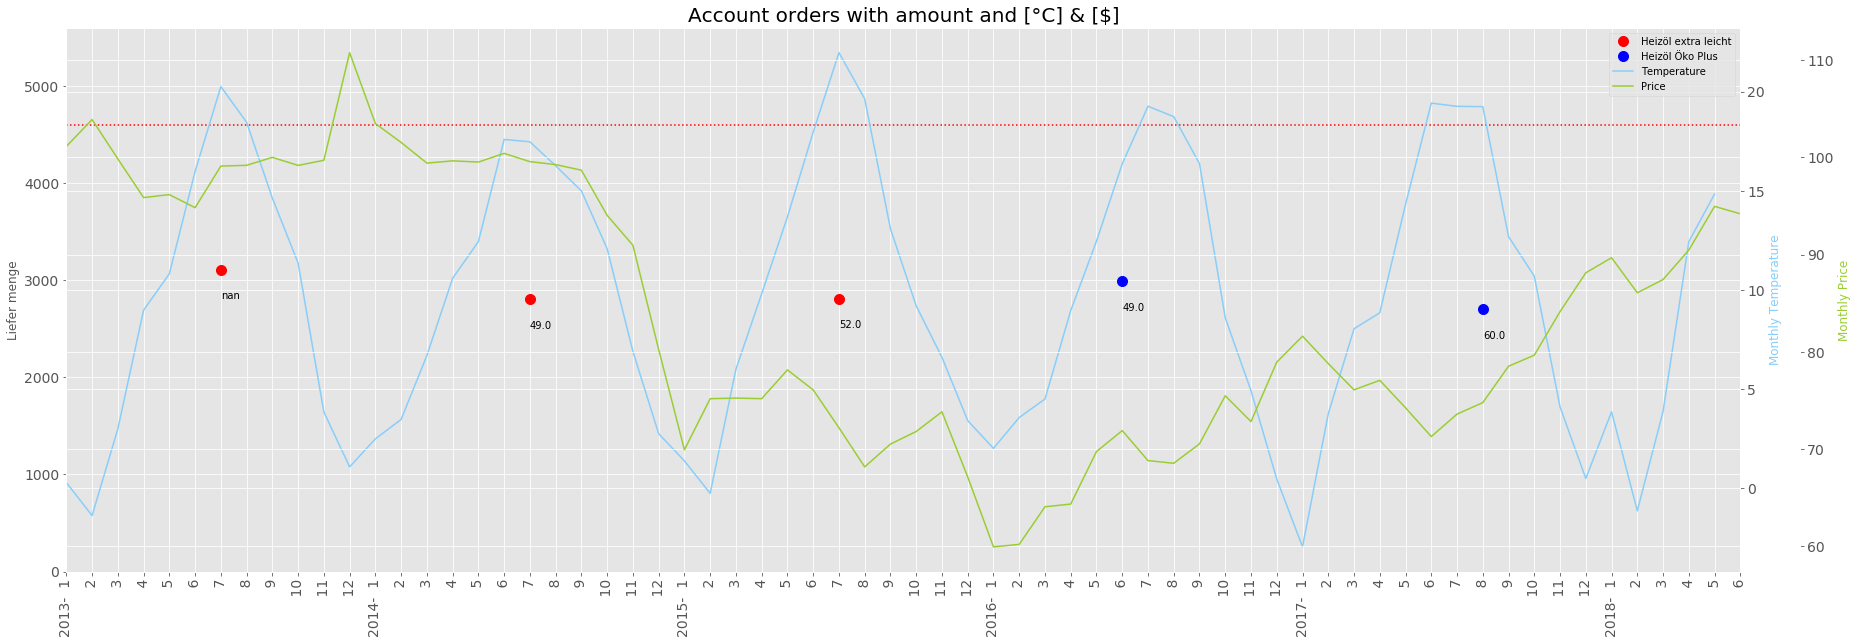
\includegraphics[width=20cm]{images/customer-journey.png}
    \caption{Example of a customer journey plot}
    \label{fig-annex:customer-journey}
\end{figure}



% --------------- NN experiments
\chapter{Neural Network experiments}
\label{annex:nn-experiments}

\textbf{Sketch of a simple neural network:}
\begin{figure}[h]
    \centering
    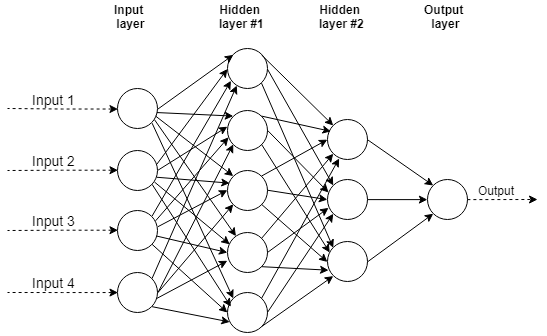
\includegraphics[width=10cm]{images/nn-sketch.png}
    \caption{Sketch a the Neural Network architecture composed of fully-connected layers.}
    \label{fig-annex:nn-sketch}
\end{figure}

\textbf{Models used:}\\
\texttt{Model 1}: One hidden layer composed of 90 neurons. \\
\texttt{Model 2}: One hidden layer composed of 200 neurons. \\
\texttt{Model 3}: Two hidden layers composed of 90 and 30 neurons respectively. \\
\texttt{Model 4}: Three hidden layers composed of 90, 60 and 30 neurons respectively. \\
\texttt{Model 5}: Three hidden layers composed of 200, 90 and 30 neurons respectively. \\

\textbf{Set of features used:}\\
\texttt{Features 1}: Set of features composed of the entire XXX features created. \\
\texttt{Features 2}: Set of 41 features related to account, previous order and current month with price and weather data. \\
\texttt{Features 3}: Set of 20 features similar to set 2 but without account features. \\
\texttt{Features 4}: Set of 10 features related to account, previous order and current month but without price and weather information. \\
\texttt{Features 5}: Set of 23 features similar to set 4 but with price and weather data. \\
\texttt{Features 6}: Set of 16 features similar to set 4 but with price data. \\
\texttt{Features 7}: Set of 19 features similar to set 4 but with weather data. \\

\textbf{Results:}
\begin{table}[!h]
    \centering
    \begin{tabular}{c|c|c|c|c|c}
        \textbf{Model} & \textbf{Features} & \textbf{Best epoch} & \textbf{Precision} & \textbf{Recall} & \textbf{F1-score} \\ \hline
        Model 5     &   	Features 5      &   	6       &   	0.8029  &   	0.8029  &   	0.8029  \\
        Model 4     &   	Features 4      &   	8       &   	0.8028  &   	0.8028  &   	0.8028  \\
        Model 5     &   	Features 4      &   	7       &   	0.8027  &   	0.8027  &   	0.8027  \\
        Model 4     &   	Features 5      &   	6       &   	0.7988  &   	0.7988  &   	0.7988  \\
        Model 5     &   	Features 7      &   	9       &   	0.7984  &   	0.7984  &   	0.7984  \\
        Model 5     &   	Features 6      &   	7       &   	0.7966  &   	0.7966  &   	0.7966  \\
        Model 4     &   	Features 7      &   	8       &   	0.7946  &   	0.7946  &   	0.7946  \\
        Model 4     &   	Features 6      &   	7       &   	0.7914  &   	0.7914  &   	0.7914  \\
        Model 2     &   	Features 4      &   	9       &   	0.7810  &   	0.7810  &   	0.7810  \\
        Model 2     &   	Features 7      &   	4       &   	0.7805  &   	0.7805  &   	0.7805  \\
        Model 3     &   	Features 5      &   	6       &   	0.7776  &   	0.7776  &   	0.7776  \\
        Model 1     &   	Features 4      &   	6       &   	0.7759  &   	0.7759  &   	0.7759  \\
        Model 3     &   	Features 4      &   	7       &   	0.7752  &   	0.7752  &   	0.7752  \\
        Model 1     &   	Features 7      &   	7       &   	0.7749  &   	0.7749  &   	0.7749  \\
        Model 2     &   	Features 5      &   	8       &   	0.7741  &   	0.7741  &   	0.7741  \\
        Model 1     &   	Features 5      &   	9       &   	0.7718  &   	0.7718  &   	0.7718  \\
        Model 3     &   	Features 7      &   	8       &   	0.7704  &   	0.7704  &   	0.7704  \\
        Model 5     &   	Features 1      &   	0       &   	0.7669  &   	0.7669  &   	0.7669  \\
        Model 2     &   	Features 6      &   	8       &   	0.7650  &   	0.7650  &   	0.7650  \\
        Model 3     &   	Features 6      &   	4       &   	0.7632  &   	0.7632  &   	0.7632  \\
        Model 1     &   	Features 6      &   	6       &   	0.7611  &   	0.7611  &   	0.7611  \\
        Model 5     &   	Features 2      &   	0       &   	0.7513  &   	0.7513  &   	0.7513  \\
        Model 4     &   	Features 2      &   	9       &   	0.7425  &   	0.7425  &   	0.7425  \\
        Model 4     &   	Features 1      &   	0       &   	0.7360  &   	0.7360  &   	0.7360  \\
        Model 2     &   	Features 2      &   	4       &   	0.7218  &   	0.7218  &   	0.7218  \\
        Model 1     &   	Features 2      &   	8       &   	0.7190  &   	0.7190  &   	0.7190  \\
        Model 1     &   	Features 1      &   	1       &   	0.7168  &   	0.7168  &   	0.7168  \\
        Model 3     &   	Features 2      &   	3       &   	0.7142  &   	0.7142  &   	0.7142  \\
        Model 2     &   	Features 1      &   	0       &   	0.7124  &   	0.7124  &   	0.7124  \\
        Model 3     &   	Features 1      &   	0       &   	0.6822  &   	0.6822  &   	0.6822  \\
        Model 5     &   	Features 3      &   	5       &   	0.5581  &   	0.5581  &   	0.5581  \\
        Model 3     &   	Features 3      &   	1       &   	0.5222  &   	0.5222  &   	0.5222  \\
        Model 2     &   	Features 3      &   	2       &   	0.5159  &   	0.5159  &   	0.5159  \\
        Model 4     &   	Features 3      &   	5       &   	0.5143  &   	0.5143  &   	0.5143  \\
        Model 1     &   	Features 3      &   	3       &   	0.5007  &   	0.5007  &   	0.5007  \\
    \end{tabular}
    \caption{Results for the model's architecture and features experiments. Scores retrieved with the testing dataset. Table sorted by decreasing Testing F1-score.}
    \label{tab-annex:nn-experiments}
\end{table}


\textbf{Comments:}\\
Bla bla bla



% --------------- NN fine-tuning results
\chapter{Neural Network fine-tuning results}
\label{annex:nn-fine-tuning}

The fine-tuning phase is decomposed into four parts, each part related to a parameter.

Note that on the results below, the F1-score is decreasing some times, even by keeping the best configuration. This is a well known issue when using Keras model: there is still some part of randomness that cannot be fixed, even with seed! REF REF REF

\begin{enumerate}
    \item Activation function
        \begin{table}[!h]
            \centering
            \begin{tabular}{c|c|c|c|c|c}
            \textbf{Activation function} & \textbf{Precision} & \textbf{Recall} & \textbf{F1-score} \\ \hline
            Linear      &   	0.8029  &   	0.8029  &   	0.8029  \\
            tanh        &   	0.8028  &   	0.8028  &   	0.8028  \\
            softmax     &   	0.8027  &   	0.8027  &   	0.8027  \\
            elu         &   	0.8029  &   	0.8029  &   	0.8029  \\
            softmax     &   	0.8028  &   	0.8028  &   	0.8028  \\
            relu        &   	0.8027  &   	0.8027  &   	0.8027  \\
            selu        &    	0.8029  &   	0.8029  &   	0.8029  \\
            softplus    &   	0.8028  &   	0.8028  &   	0.8028  \\
            softsign    &   	0.8027  &   	0.8027  &   	0.8027  \\
            sigmoid     &   	0.8029  &   	0.8029  &   	0.8029  \\
            hard sigmoid        &   	0.8028  &   	0.8028  &   	0.8028  \\
            \end{tabular}
            \caption{Results the fine-tuning of the activation function. Scores retrieved with the testing dataset.}
        \end{table}
    
    \item Loss function
        \begin{table}[!h]
            \centering
            \begin{tabular}{c|c|c|c|c|c}
                \textbf{Loss function} & \textbf{Precision} & \textbf{Recall} & \textbf{F1-score} \\ \hline
                mean absolute error      &   	0.8029  &   	0.8029  &   	0.8029  \\
                mean squarred error        &   	0.8028  &   	0.8028  &   	0.8028  \\
                mape     &   	0.8027  &   	0.8027  &   	0.8027  \\
                msle         &   	0.8029  &   	0.8029  &   	0.8029  \\
                kid     &   	0.8028  &   	0.8028  &   	0.8028  \\
                cosine        &   	0.8027  &   	0.8027  &   	0.8027  \\
                categorical hinge        &    	0.8029  &   	0.8029  &   	0.8029  \\
                logcosh    &   	0.8028  &   	0.8028  &   	0.8028  \\
            \end{tabular}
            \caption{Results the fine-tuning of the loss function. Scores retrieved with the testing dataset.}
        \end{table}
        
        
    \item Optimizer
        \begin{table}[h]
            \centering
            \begin{tabular}{c|c|c|c|c|c}
                \textbf{Optimizer} & \textbf{Precision} & \textbf{Recall} & \textbf{F1-score} \\ \hline
                adam      &   	0.8029  &   	0.8029  &   	0.8029  \\
                sgd        &   	0.8028  &   	0.8028  &   	0.8028  \\
                rmsprop     &   	0.8027  &   	0.8027  &   	0.8027  \\
                adagrad         &   	0.8029  &   	0.8029  &   	0.8029  \\
                adamax     &   	0.8028  &   	0.8028  &   	0.8028  \\
            \end{tabular}
            \caption{Results the fine-tuning of the optimizer choice. Scores retrieved with the testing dataset.}
        \end{table}


    \item Bias usage
        \begin{table}[h]
            \centering
            \begin{tabular}{c|c|c|c|c|c}
                \textbf{Bias} & \textbf{Precision} & \textbf{Recall} & \textbf{F1-score} \\ \hline
                True      &   	0.8029  &   	0.8029  &   	0.8029  \\
                False        &   	0.8028  &   	0.8028  &   	0.8028  \\
            \end{tabular}
            \caption{Results the fine-tuning for the bias usage. Scores retrieved with the testing dataset.}
        \end{table}
        
        
    \end{enumerate}


% --------------- LSTM results
\chapter{LSTM experiments}
\label{annex:lstm-experiments}